\documentclass[tikz, dvipsnames]{standalone}

\usetikzlibrary{positioning}

\usetikzlibrary{calc}
\begin{document}
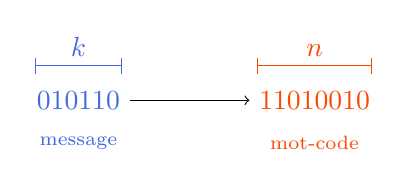
\begin{tikzpicture}
\node[RoyalBlue] (A) at (0,0) {010110};
\node[OrangeRed] (B) at (3,0) {11010010};
\draw[|-|,RoyalBlue] ($(A.north west)+(1mm,2mm)$) -- ($(A.north east)+(-1mm,2mm)$) node[midway,anchor=south] (C) {$k$};
\draw[|-|,OrangeRed] ($(B.north west)+(1mm,2mm)$) -- ($(B.north east)+(-1mm,2mm)$) node[midway,anchor=south] (D) {$n$};
\node[anchor=south] at (0,-0.75) {\scriptsize \textcolor{RoyalBlue}{message}};
\node[anchor=south] at (3,-0.75) {\scriptsize \textcolor{OrangeRed}{mot-code}};
\draw[->] (A) -- (B);
\end{tikzpicture}
\end{document}